\chapter{Research Methodology}
\label{chap:method}
This chapter presents the research methodology used in this thesis. Firstly, the research motivation is presented in \cref{sec:research-motivation}, followed by the research questions defined for this thesis in \cref{sec:research-questions}. The research method and design are explained in \cref{sec:research-method-and-design}. Then, \cref{sec:design-for-rq1,sec:design-for-rq2} presents the research design for RQ1 and RQ2, respectively. \cref{sec:project-scope} describes the project scope. Finally, \cref{sec:technology} presents the various software libraries and hardware used in this thesis.

\section{Research Motivation}
\label{sec:research-motivation}
Writing Smart Contracts are hard. Writing secure Smart Contracts is even harder. Automatic code generation is by many considered the ”holy grail” in the field of computer science \cite{PGL-010}. Ever since OpenAI introduced its first transformer model in the GPT series, this class of transformers has been touted as the state-of-the-art for text generation. Recent works have applied transformers for code generation and program synthesis, achieving state-of-the-art results. For example, Codex by \cite{chen2021codex} fine-tunes GPT-3 \cite{brown2020language} on code data from GitHub. The results are impressive. However, these systems still face many problems, especially in regards to different biases, for example, gender and security biases. Because the model is trained on open-source code \cite{chen2021codex}, including "Public code may contain insecure coding patterns, bugs, or references to outdated APIs or idioms.", the model might "synthesize code that contains these undesirable patterns introduce vulnerabilities" \cite{copilot}. An empirical study by \textcite{pearce2021asleep} found that almost approximately 40\% of the generated code by GitHub Copilot is vulnerable. Security flaws in software results yearly in loss of tens of thousands of million dollars\todo{find real number here .}. Due to the monetary nature of blockchain, security flaws are even more severe, as exploits of vulnerabilities often directly result in the loss of funds. Further, the immutable nature prevents the possibility of correcting vulnerable code after being deployed. Therefore, the research objective is to develop a system that can generate secure smart contract code automatically, without the need for human intervention. \todo{Add comment-aided  approach arguments}. This thesis tries to address the above problems by answering the research questions defined in \cref{sec:research-questions}.

\section{Research Questions}
\label{sec:research-questions}
The research questions addressed in this thesis are:

\begin{enumerate}[label=\textbf{RQ\arabic*.}, leftmargin=1.5cm]
    \item How to automatically generate \acrlong{sc} code with transformer-based language models, by inputting comments to guide the code generation?
    \item How to generate secure \acrlong{sc} code with transformer-based language models?
    %\item How to reduce the vulnerability bias in the transformer model.
\end{enumerate}

\section{Research Method and Design}
\label{sec:research-method-and-design}

%The underlying foundation for how research is conducted is rooted in the research philosophy used. For this research, a positivistic research philosophy was used. A positivistic philosophy assumes that the world is not random, that it is ordered and regular, and that one can investigate it objectively. \cite{oates2006researching} A deductive research approach was used. \todo{Remove deductive?}

To best facilitate the answering of the research questions defined in \cref{sec:research-questions}, an \acrfull{dsr} was selected as the research approach. A \acrshort{dsr} focuses on the development and performance of artifacts. For this to be considered research, the work needs to demonstrate academic qualities such as analysis, explanation, argument, justification, and critical evaluation. Further, the work needs to contribute to knowledge in some way \cite{oates2006researching}.
\acrshort{dsr} is typically an iterative process that involves five steps \cite{vaishnavi2004design}: Awareness of Problem, Suggestion, Development, Evaluation, and Conclusion.
\begin{itemize}
    \item \textbf{Awareness of Problem}: is the recognition and formulation of a problem. This might come from multiple sources, such as areas identified by authors for further research, reading about new developments in the industry, from other disciplines, new technological developments, etc. The output of this phase is a proposal for a new research effort, either formal or informal.
    \item \textbf{Suggestion}: directly follows the development of a proposal based on an awareness of a problem. This is the creative step where a tentative idea of how to solve such a problem in a novel way is suggested.
    \item \textbf{Development}: is the actual implementation of the suggested idea. This is the step where the tentative design idea is implemented and produces an artifact. The techniques used for implementation vary with the type of artifact, which could be anything from algorithms to models.
    \item \textbf{Evaluation}: is the evaluation of the artifact. In this step, the artifact's worth is assessed, as well as potential deviations from expectations. 
    \item \textbf{Conclusion}: is the final step where the results from the design process are determined to be "good enough". The results are written up. The knowledge gained is identified, along with any loose ends that might serve as subjects for future research.
\end{itemize}

\noindent
For this thesis, \cref{sec:research-motivation} clearly describes the awareness of the problems this thesis aims to solve. This is the motivation behind the new research effort proposed in this thesis, conveyed as research questions defined in \cref{sec:research-questions}. The following sections;\todo{Check : or ;} \cref{sec:design-for-rq1} and \cref{sec:design-for-rq2} describe a suggestion for how to solve these research questions. \cref{chap:implementation-and-results} describes the implementation of the suggested solution for the research questions, while \cref{chap:evaluation} presents an evaluation of the implementation results. Finally, the findings and results are discussed in \cref{chap:discussion}, and areas suitable for further research are presented in \cref{chap:future-work}.
%
%The next section describes the suggestion step. The next section describes the development step. The next section describes the %evaluation step. The next section describes the conclusion step.
%This thesis aims to solve the research questions defined in \cref{sec:research-questions}. 
%
%These experiments included fine-tuning pre-trained language models, as well as testing these on real data and man-made data. The %results from the evaluation of the fine-tuned models are recorded as observations and quantitatively evaluated.
%
%This project employs . \acrfull{dsr} is a ... 



%The research is conducted objectively. It is based on facts that are repeatable and quantitatively evaluated. 


%Research Philosophy - positivism
%Research Type - inductive (exploratory) + Quantitative
%Research Strategy - experiments (train and test)
%Time Horizon- one-time data set construction (1st of april)
%Sampling Strategy  - probability sampling (random)
%Data Collection Method - Observation? Evaluate performance
%Data Analysis Methods - Employ primarily a quantitative analysis, as well as some qualitative analysis. (mixed methods?)


%\section{Research Implementation}
%\label{sec:research-implementation}
%
%For the implementation of the research, first, the datasets needed for the experiments were constructed. The datasets creation %phase is divided into the following steps:
%\begin{enumerate}
%    \item Create verified smart contract source code dataset.
%    \begin{enumerate}
%        \item Scrape verified smart contracts from the Ethereum blockchain.
%        \item Filter scraped verified smart contracts for uniqueness.
%    \end{enumerate}
%    \item Create an audited version of the smart contract dataset
%    \begin{enumerate}
%        \item Label the smart contracts with a vulnerability detection tool.
%    \end{enumerate}
%    \item Create a parsed dataset containing "comment, function" pairs. This will facilitate testing, as well as research %question 3.
%    \begin{enumerate}
%        \item Create a parser that can parse all contract versions.
%        \item Parsing the verified smart contracts with a parser.
%    \end{enumerate}
%\end{enumerate}
%A comprehensive description of the creation of the datasets used in this project is given in \cref{chap:datasets}.
%\newline
%\newline
%Secondly, the language modeling process is divided into 2 phases:
%\begin{enumerate}
%    \item Fine-tune a transformer model on the verified smart contracts dataset.
%    \item Fine-tune a transformer model on the audited verified smart contract dataset, employing security conditioning.
%\end{enumerate}
%A comprehensive description of the implementation of the language models is given in \cref{chap:language-modeling}.


\section{Design for RQ1}
\label{sec:design-for-rq1}
This section describes the design for research question 1. For constructing a comment-aided system for automatically generating smart contract code, multiple design steps are needed. The first subsection describes how comment The following subsections describe a system that can generate secure smart contract code automatically, this project uses a deep learning approach. Further, for understanding how to put this system to use in a comment-driven approach, a comment analysis is conducted.

\subsection{Code comments analysis}
\label{sec:code-comments-analysis}
\todo{Add a description of the code comments analysis. + the differrent types of comments. + different styles?}
It is tehrefore needed to analyze the comments in order to investigate how a user can best use this auto-generating system.

\subsection{Language Model}
\label{sec:language-model}
As discussed in section \cref{sec:transformers-for-code-synthesis}, there are several available transformer models. However, only a few of them have open-sourced pre-trained weights. Of these, GPT-J \cite{gpt-j} is the largest model that includes code in its pre-training dataset "The Pile", described in \cref{sec:the-pile}. The research community has found these models to outperform existing open-source GPT systems in qualitative programming evaluations \cite{wolf2021}. These findings are further backed by \cref{chen2021codex}. Because of this, the state-of-the-art generative pre-trained transformer model GPT-J is the language model used in this thesis.

\subsubsection{Model architecture}
\label{sec:architecture}
Ever since OpenAI introduced its first transformer model in the GPT series, this class of transformers has been touted as the state-of-the-art for text generation. Their latest model, GPT-3 \cite{brown2020language}, is their best performing model with 175 billion parameters. However, the model is not openly available at the current time. GPT-J \cite{gpt-j} with 6 billion parameters (GPT-J-6B) is currently one of the best open-source alternatives to OpenAI's GPT-3. GPT-J was released in June 2021 by EleutherAI \cite{elutherai}, a grassroots collection of researchers working to open-source AI research. The model is trained on the Pile, an 825 GiB diverse, open-source language modeling data set that consists of 22 smaller, high-quality datasets combined together. See section \cref{sec:the-pile} for a more detailed description of the Pile.

Being a GPT class transformer, GPT-J uses a decoder-only architecture, as can be seen in \cref{fig:gpt-j-architecture}. The GPT-J introduces some notable differences from standard transformer models. Firstly, instead of computing attention and feed-forward layers in sequential order, they are computed in parallel and the results are added together. This decreases communication during distributed training, resulting in increased throughput. Secondly, GPT-J uses \acrfull{rope} \cite{su2021roformer} for position encoding. Opposite to sinusoidal encoding used in standard transformer models (see \cref{sec:embedding-and-positional-encoding}), this is shown to result in better model quality in tasks with long text \cite{su2021roformer}.

\begin{figure}[htbp]
    \centering
    %\def\svgwidth{\linewidth}
    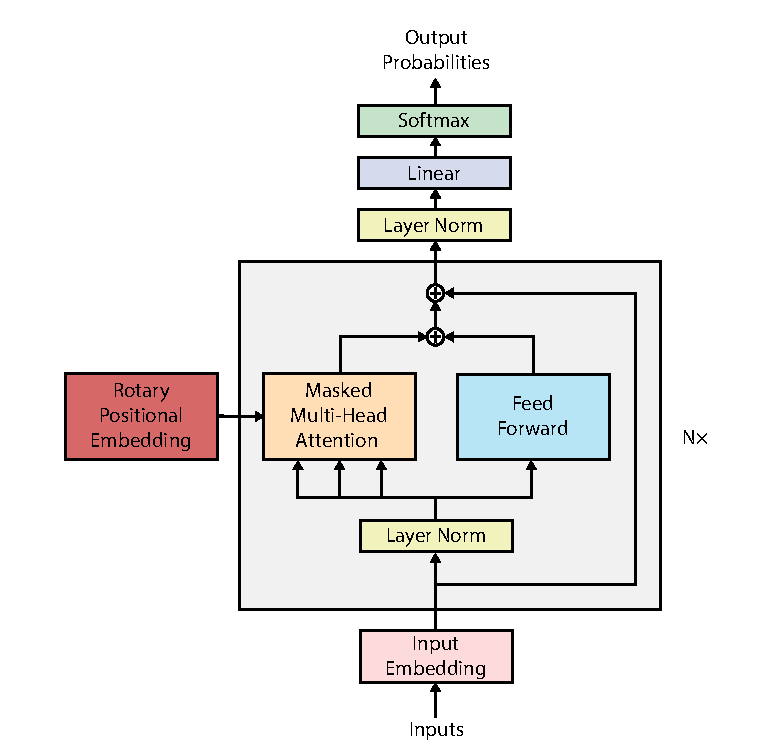
\includegraphics[width=0.8\textwidth]{figures/gpt-j_architecture.pdf}
    \caption{Diagram of GPT-J model architecture.}
    \label{fig:gpt-j-architecture}
\end{figure}

\subsubsection{Requirements}
\label{sec:requirements}
To load the GPT-J model in float32 precision, one would need at least 2x the model size of CPU RAM: 1x for the initial weights and another 1x to load the checkpoint. So for just loading the GPT-J model, it would require at least 48GB or CPU RAM. To reduce the memory footprint, one can load the model in half-precision.

GPU needs around 40GB of GPU memory to load the model. For training/fine-tuning the model, it would require significantly more GPU RAM. For example, the Adam optimizer makes four copies of the model: model, gradients, average and the squared average of gradients. Hence, it would take 4x model size GPU memory, even with mixed precision as gradient updates are in fp32. Further, this doesn't include the activations and data batches which would require some more GPU RAM. Hence, solutions like DeepSpeed needs to be used for training/fine-tuning such large models.

If a GPU with mixed precision capabilities (architecture Pascal or more recent) is available, one can use mixed precision training with PyTorch 1.6.0 or later, or by installing the Apex library for previous versions. If using an NVIDIA “Ampere” GPU architecture, the \acrfull{bf16} floating-point format can be used. Using mixed precision training usually results in 2x-speedup for training with the same final results.

\subsubsection{Pre-training}
Pre-training is defined as "Training in advanced". By first training the model on a huge dataset, the model can then be fine-tuned on a much smaller dataset. This is so-called transfer learning. The pre-training procedure used for GPT class models is called \acrshort{clm}. The model reads the text input in order and then tries to predict the next word. The model is fed a complete text element (input sequence) all at once, and then internal masking is applied to prevent the model from cheating by looking at future tokens. For more details on the inner workings of the training procedure, see \cref{sec:transformer-training}.

\subsubsection{The Pile}
\label{sec:the-pile}
Describe the  PILE...  It consists of among others, a lot of data from GitHub. However, only x\% of the data is smart contracts (Solidity). Hence there is a need for a dataset made up of smart contracts. --> existing datasets....

\begin{figure}[htp]
    \centering
    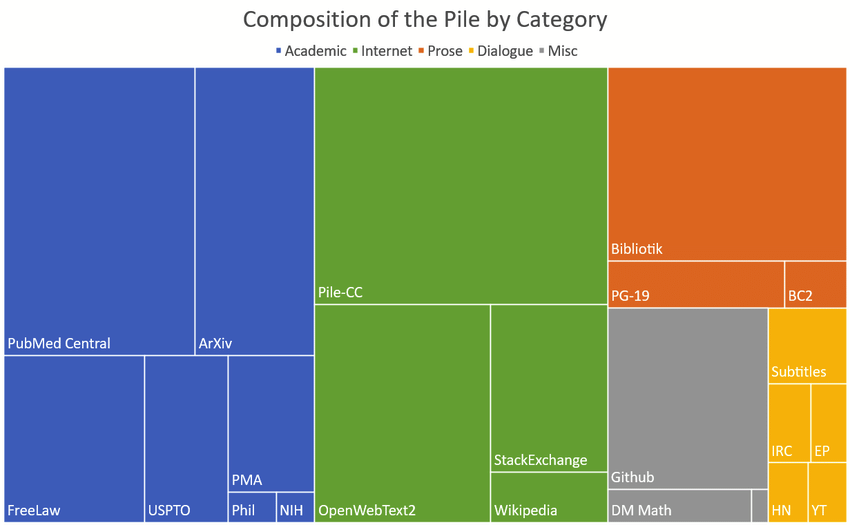
\includegraphics[width=\textwidth]{figures/Treemap-of-Pile-components-by-effective-size.png}
    \caption{Treemap of Pile components by effective size. SOURCE FROM THEPILE paper}
    \label{fig:flowchart}
\end{figure}

\subsection{Metrics}
For evaluating the model performance, the accuracy and perplexity metrics are used. For evaluating the function  genertion from comments, the bleu score will be used. See \label{sec:rq1-evaluation-metrics}.
\todo{Do i need this section? }

\section{Design for RQ2}
\label{sec:design-for-rq2}
Use secure vs vulnerabile as input to the  model inorder to generate secure code. 
Why might this idea work? Justify.

\subsection{Security Conditioning}
\label{sec:security-conditioning}
\todo{Rewrite - this is a draft}
When training a large language model on several gigabytes of open-source code, it is safe to assume that large portions of this code are not safe and contains vulnerabilities. In the case of Smart Contracts, the vulnerability analysis presented in section \ref{sec:verified-smart-contracts} shows that almost 50\% of deployed Smart Contracts contain at least one high-severity vulnerability. This will result in a biased model that may produce a lot of vulnerable code. This section introduces a technique, named security conditioning, to reduce and mitigate this problem.

Vulnerability analysis is a difficult area. It is especially hard in the area of smart contracts, where the execution environment is not deterministic ????\todo{find correct wording.}... Previous works have tried to classify vulnerable code with large language models without much success \todo{Cite previous works}. In this project, instead of classifying vulnerable code, the goal is to make the model more secure by conditioning it on the presence of vulnerabilities.

The security conditioning is done by appending a special security label to each of the records in the training data. This way, the model can use this token(s) to condition whether to produce safe or vulnerable code. This requires the dataset to first be labeled as secure or vulnerable. For this project, SolidityDetector is used for labeling. Further details on the dataset construction can be found in \cref{sec:verified-smart-contracts-audit}.

\subsection{Metrics}
For evaluating the model has not droppedin performance, the  accuracy and perplexity  metrics are used. 
\todo{Do i need this section? }

\section{Project scope}
\label{sec:project-scope}

The project scope in this thesis is limited to the generation of smart contracts for the Ethereum blockchain. Further, only one language model architecture is used. Specifically, the state-of-the-art open-sourced pre-trained transformer model GPT-J-6B by ElutherAI is selected. For research questions 1 and 2, two versions of the model were created by fine-tuning it on two smart contract datasets created for this project. Due to the share size of this model (see \cref{sec:requirements}), no hyper-parameter optimization was performed. The hyper-parameters were left to defaults used during pre-training. Hence, everything but the training data is kept constant throughout the experiments. For research question 3, the primary scope is to assess variations in the actual input to the model. Thus, differences in performance due to variations of the models' inference configuration are not thoroughly explored.

Several options are available for tuning the code generation, including \textit{temperature}, \textit{stops}, and \textit{top p}.

\todo{Restricted to mainly Solidity language}

\section{Technology}
\label{sec:technology}
Following is an overview of the different technologies applied in this project, both software and hardware.

\subsection{Software}
\label{sec:software}
During the selection of the language modeling library for use in this project, several considerations were made. Firstly, due to the huge size of the model, the library needed to support distributed GPU training. It had to be flexible and scalable, without sacrificing too much on speed. The transformers \cite{transformers} library by Hugging Face \cite{huggingface} fulfilled these conditions. The library provides flexible and easy-to-use solutions. It also supports integration with DeepSpeed \cite{deepspeed}, a deep learning optimization library by Microsoft \cite{microsoft} that makes distributed training and inference easy, efficient, and effective. The Hugging Face ecosystem also provides the Datasets and Tokenizers libraries, streamlining and significantly simplifying the use of large datasets.

NLTK, extensive use of Pandas, as well as Pytorch, Numpy, and Matplotlib are used for data processing and visualization. For traching training experiments, WANDB is used.\todo{Fix}

\paragraph{DeepSpeed}
\label{par:deepspeed}
The deep learning optimization library DeepSpeed \cite{deepspeed} is used for training. It facilitates both distributed training, mixed precision and gradient accumulation, providing significant speedup of the training process while still being able to fit the model into the GPU memory available. The main workhorse of DeepSpeed is the \acrfull{zero} \cite{zero}. \acrshort{zero} comes with three incremental optimization stages: stage 1 (\acrshort{zero}-1), stage 2(\acrshort{zero}-2) and stage 3(\acrshort{zero}-3).

\begin{itemize}
    \item \textbf{Stage 1}: partitions the optimizer states across the processes, so each process only updates its partition.
    \item \textbf{Stage 2}: partitions the reduced gradients for updating the model weights, so that each process only retains the gradients corresponding to its own portion of the optimizer states.
    \item \textbf{Stage 3}: partitions the model parameters across the processes. They are automatically collected and partitioned during forward and backward passes.
\end{itemize}

\noindent
For training exceptionally large models, DeepSpeed also provides heterogeneous memory technologies based on \acrshort{zero}. This includes \acrshort{zero}-Offload for \acrshort{zero}-2 and \acrshort{zero}-Infinity \cite{zeroinfinity} for \acrshort{zero}-3. \acrshort{zero}-Offload offloads the optimizer memory and computation from the GPU to the host CPU. \acrshort{zero}-Infinity is an upgraded version of \acrshort{zero}-Offload that also allows for offloading to \gls{nvme} memory. DeepSpeed \acrshort{zero} makes it possible to train trillion parameter models \cite{zeroinfinity}. However, each optimization stage comes with a performance cost, slowing down the training process. DeepSpeed also provides support for mixed-precision training \cite{mixedprecision}. Mixed-precision training is the use of lower-precision operations (\acrshort{fp16} and \acrshort{bf16}) in a model during training. This both makes it run faster and uses less memory.

\subsection{Hardware resources}
\label{sec:hardware-resources}

IDUN High Performance Computing Platforms \cite{epic}.
IDUN full-fills the requirements defined in \cref{sec:requirements}.
\todo{Describe more in detail}
\begin{figure}[htp]
    \centering
    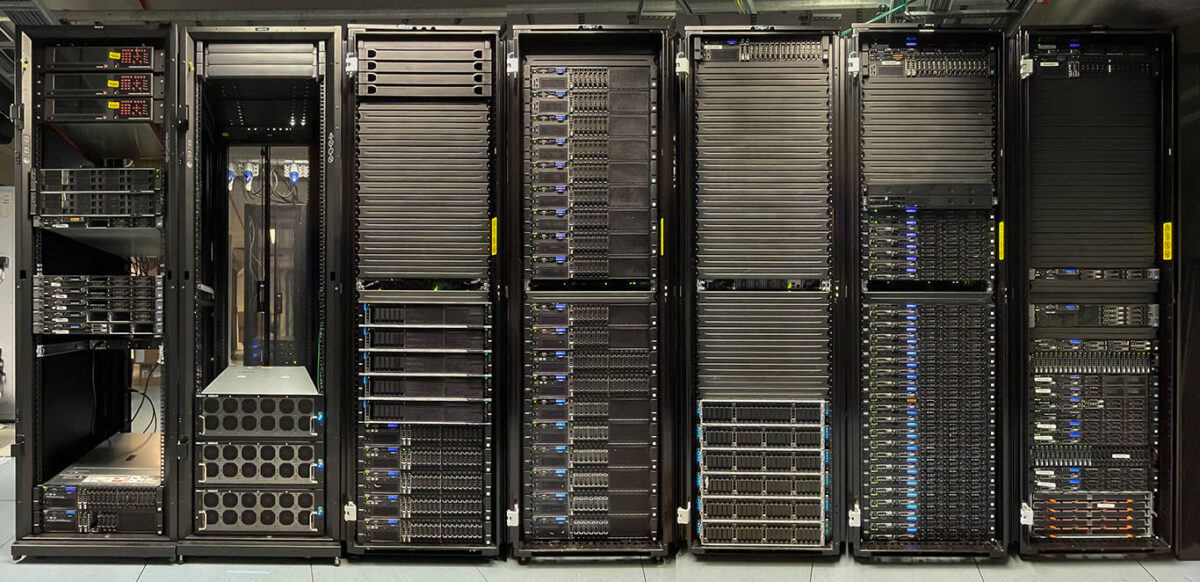
\includegraphics[width=\textwidth]{figures/idun.jpeg}
    \caption{Image of IDUN todo: add ref \url{https://www.hpc.ntnu.no/idun/}}
    \label{fig:flowchart}
\end{figure}
